\begin{theorem}
  If $X$ is an irreducible topological space and $\Sh{F}$ is a constant sheaf, then $H^r(X, \Sh{F})$ for all $r>0$.
\end{theorem}
\begin{proof}
  Since any open set $U \subseteq X$ is connected, $\Sh{F}(U) = G$ if $\Sh{F}$ is the constant sheaf defined by the group $G$ and $U$ is nonempty. This means that $\Sh{F}$ is flasque, hence $H^r(X, \Sh{F})$ for all $r>0$.
\end{proof}
It follows that constant sheaves on varieties have no higher cohomology. The reason ist that there are not enought open sets in the Zariski topology. In order to fix this, we introduce the notion of \'etale morphism, which will allow us to consider sheaves on a larger category $\acute{Et}/X$ instead of the category of open sets of $X$. This category bears a strong resemblence to the category of open sets, but contains as objects not open sets but \textit{local homeomorphisms}.

As we have seen, sheaves relate the local and global information one has on a given topological space $X$. In a sense sheaf cohomology measures how much more information we gain when we go from global to local. For example, consider the sheaf of local sections of the covering space $\pi : X \to S^1$.

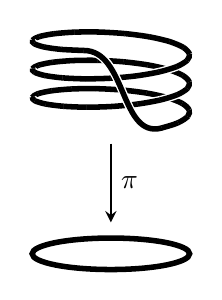
\begin{tikzpicture}[declare function={f(\x)=0.2*sin(\x)+\x/1000;},
  rubout/.style={/utils/exec=\tikzset{rubout/.cd,#1},
  decoration={show path construction,
       curveto code={
        \draw [white,line width=\pgfkeysvalueof{/tikz/rubout/line width}+2*\pgfkeysvalueof{/tikz/rubout/halo}] 
         (\tikzinputsegmentfirst) .. controls
         (\tikzinputsegmentsupporta) and (\tikzinputsegmentsupportb)  ..(\tikzinputsegmentlast); 
        \draw [line width=\pgfkeysvalueof{/tikz/rubout/line width},shorten <=-0.1pt,shorten >=-0.1pt] (\tikzinputsegmentfirst) .. controls
         (\tikzinputsegmentsupporta) and (\tikzinputsegmentsupportb) ..(\tikzinputsegmentlast);  
       }}},rubout/.cd,line width/.initial=2pt,halo/.initial=0.5pt]
  \draw[rubout={line width=2pt,halo=0.5pt},decorate] 
    plot[variable=\x,domain=-50:970,samples=55,smooth] ({cos(\x)},{f(\x)}) to[out=0,in=195] cycle;
  \draw[line width=2pt] (0,-2) arc(-90:270:1cm and 0.2cm);
  \draw[thick,-stealth]  (0,-0.4) -- (0,-1.4) node[midway,right]{$\pi$};
 \end{tikzpicture} 

There is no global section $s: S^1 \to X$ but locally, the set of sections $\{s: U \to \pi^{-1}(U) | \pi \circ s = id$ is a set with three elements.

Let $X$ be a topological space. A theorem of algebraic topology says that for any abelian group $A$, the cohomology group $H^1(X,A)$ with coefficients in $A$ is isomorphic to the abelianisation of the fundamental group $\pi_1(X)$